\documentclass{beamer}
\usepackage{wasysym}

\usepackage[framemethod=tikz]{mdframed}
\usepackage[makeroom]{cancel}
\usepackage{tikz}

\setbeamercolor{background canvas}{bg=white}

\tikzstyle{every picture}+=[remember picture]
\usetikzlibrary{arrows,positioning}
\tikzset{
	%Define standard arrow tip
	>=stealth',
	%Define style for boxes
	punkt/.style={
		rectangle,
		rounded corners,
		draw=black, very thick,
		text width=6.5em,
		minimum height=2em,
		text centered},
	% Define arrow style
	pil/.style={
		->,
		thick,
		shorten <=2pt,
		shorten >=2pt,}
}
\usetikzlibrary{positioning}

\usetheme[sectionpage=none,numbering=counter]{metropolis}
%\setbeamertemplate{footline}[frame number]
\usepackage{graphicx}
\usepackage[utf8]{inputenc}
\usepackage[T1]{fontenc} 
\newcommand{\textoverscript}[1]{$^{\text{#1}}$}
\newcommand{\textunderscript}[1]{$_{\text{#1}}$}
\usepackage{caption}
\captionsetup{justification=raggedright,singlelinecheck=false}
\captionsetup[figure]{labelformat=empty}


\setbeamercovered{transparent}% Dim out "inactive" elements
\setbeamertemplate{caption}{\raggedright\insertcaption\par}
\setlength\abovecaptionskip{-15pt}
\newcommand{\tabitem}{%
  \usebeamertemplate{itemize item}\hspace*{\labelsep}}
\title{Velocity Distribution Functions of Pickup Ions with Ulysses/SWICS}
\subtitle{Master Thesis}
%\subtitle{MNF-phys-1321 -- Methodenkenntnisse und Projektplanung}
\author{Anne Fischer}
\date{\today}
%
%
%
\begin{document}
%%%
\begin{frame}[plain]
	\titlepage
\end{frame}
%%%
\begin{frame}[plain]{Outline}
	%To Do: \\ Motivation: Understanding the VDF of He$^+$ Pickup Ions with Ulysses SWICS
	
	\tableofcontents
\end{frame}
%%%
\section{Pickup Ions}
\subsection{Basics}
\begin{frame}{Pickup Ions Basics}
	\begin{block}{ }
		\textbf{Pickup Ions: \\
			Former neutrals that get ionised within the heliosphere}
	\end{block}

	Origin of the neutrals:
	\begin{columns}
	\column{5cm}
		\begin{itemize}
			\item LISM
		\end{itemize}
		\vspace{-0.7cm}
		\begin{figure}									
			\includegraphics[scale=0.22]{Pics/lism.png}
			\caption{\tiny{\begin{center}
						\textit{from http://science.nasa.gov}
			\end{center}}}
		\end{figure}
	\column{5cm}
%	\vspace{-0.2cm}
			\begin{itemize}
		\item Inner Source
	\end{itemize}
		\begin{figure}									
			\includegraphics[scale=0.17]{Pics/inner_source.png}
			\caption{\tiny{\begin{center}
						\textit{Taut 2018}
			\end{center}}}
		\end{figure}
	\end{columns}
\end{frame}
%%%
\begin{frame}{The Pickup Process}
	\begin{figure}									
		\includegraphics[scale=0.25]{Pics/PU_process.pdf}
		\caption{\begin{flushright}
				\tiny{\textit{Taut, Drews et al., AGU fall meeting 2014}}
		\end{flushright}}
	\end{figure}
\vspace{-2.2cm}
\begin{columns}
	\column[]{4cm}
	Ionisation by:
	\begin{itemize}
		\item Photoionisation
		\item Charge exchange 
		\item Electron impact
	\end{itemize}
\vspace{2.2cm}
	\column[]{6cm}
	\textbf{$\rightarrow$ Newborn ion is subjected to\\ \hspace{0.7cm}electromagnetic forces}
\end{columns}
\end{frame}
%
%
%
\subsection{Velocity Distribution Function}
\begin{frame}{The Pickup Process}
	\begin{columns}
		\column{5.5cm}
		\vspace{0.5cm}
		\flushright
		\begin{figure}
			\includegraphics[scale=0.3]{Pics/pu_process_1_2.png}
			%\hspace{1cm}
			\caption{\begin{center}
					\tiny{Taut, Drews et al., AGU Fall Meeting 2014}
			\end{center}}
		\end{figure}
		\column{5cm}
		\only<1>{Assumptions:
			\begin{itemize}
				\item particle at rest
				\item $\vec{B} \perp \vec{v}_{SW}$
			\end{itemize}
			\vspace{1cm}
			\textbf{	Relative motion \\
				$\rightarrow$ Gyro-motion }}
		\only<2>{
			
			\begin{center}
				\textbf{Velocity Space:}
			\end{center}
			\vspace{-0.5cm}
			\begin{figure}									
				\includegraphics[scale=0.22]{Pics/injiz.png}
				\caption{\tiny{\begin{center}
							\textit{Drews et al., 2016}
				\end{center}}}
		\end{figure}
	\vspace{-1cm}
				\begin{center}
					\textbf{$\rightarrow$ Anisotropic torus VDF}	
				\end{center}
}

	\end{columns}
\end{frame}
%
%
%
\begin{frame}{Evolution of the VDF}
	\begin{figure}
		\includegraphics[scale=0.175]{Pics/torus.pdf}
		\hspace{0.001cm}
		\includegraphics[scale=0.175]{Pics/PAS.pdf}
		\hspace{0.001cm}
		\includegraphics[scale=0.175]{Pics/Cooling.pdf}
		\vspace{0.5cm}
		\caption{\tiny{\begin{flushright}
					\textit{Drews, Berger et al., 2016}
		\end{flushright}}}
	\end{figure}
	\vspace{-.5cm}
	\begin{columns}
		\vspace{.5cm}
		\column{4cm}
		Modification of the initial torus-shaped VDF by:
		\column{6cm}
		\begin{itemize}
			\item Pitch-angle scattering \\ $\rightarrow$ isotropisation
			\item acceleration \& decelaration
		\end{itemize}
	\end{columns}
%
%	
%	
\end{frame}
\begin{frame}{PUI -- Measurement}
	\begin{columns}
		\column[]{4cm}
		
		\textbf{Observed PUIs:} \\H\textoverscript{1+}, \textoverscript{3}He\textoverscript{1+}, He\textoverscript{1+}, He\textoverscript{2+}, C\textoverscript{1+}, N\textoverscript{1+}, O\textoverscript{1+}, Ne\textoverscript{1+}, Mg\textoverscript{1+}, Si\textoverscript{1+}, Fe\textoverscript{1+}
		
		\vspace{0.7cm}
		%
		\textbf{PUI or Solar Wind?}
		\begin{itemize}
			\item Charge state
			\item Velocity distribution function (VDF)
		\end{itemize}
		
		\column[]{6.5cm}
		\begin{figure}									
			\includegraphics[scale=0.25]{Pics/sw_pui_gloeckler.png}
			\caption{\begin{center}\tiny{Gloeckler et al., 1999}
			\end{center}}
		\end{figure}
	\end{columns}
\end{frame}
%%%
%

%%%
\begin{frame}{Anisotropic features of the VDF}
	\begin{columns}
		\column{4.cm}
		1D measurements discover \textbf{anisotropic features} of the VDF \\[0.5cm]
		
		\column{6cm}
		\begin{figure}									
			\includegraphics[scale=0.25]{Pics/moebius_dec.pdf}
				\caption{\begin{center}\tiny{Moebius et al., 1998}
				\end{center}}
		
		\end{figure}
	\end{columns}

\end{frame}
%%%
\begin{frame}{Anisotropic features of the VDF}
	\begin{columns}
		\hspace{-1cm}
		\column[]{3.7cm}
		\vspace{-0.2cm}
		\begin{itemize}
			\item STEREO / PLASTIC:\\ angular resolution $\rightarrow$ \\ 2D measurement
			\begin{itemize}
				\item anisotropic feature
				\item $\vec{B}$-dependency
			\end{itemize}
		\end{itemize}
		\column[]{7.5cm}
		\begin{figure}									
			\includegraphics[scale=0.22]{Pics/rvdf_9er_framed.pdf}
			\caption{\tiny{\begin{center}
						\textit{Drews, Berger et al., 2015}
			\end{center}}}
		\end{figure}
	\end{columns}
\end{frame}
%%%
\begin{frame}{Motivation}
\begin{columns}
	\column[]{5cm}
	Problem: \\ Ambiguity of 1D reduced data
	\\[1cm]
	For fully understanding the PUI transport in phase space we need to analyse the \textbf{3D velocity distribution} function
%	GRUNDSÄTZLICHES PROBLEM
%	warum 3d?
%	\begin{itemize}
%		\item Uneindeutigkeit der reduzierten 1D-Daten (unendlich viele Modellfunktionen)
%		\item einzelne Prozesse können nicht unterschieden werden
%		\item Übergang SW-frame
%	\end{itemize}
	
	\column[]{5cm}
	\includegraphics[scale=0.18]{Pics/qm.pdf}
\end{columns}

\section{Ulysses SWICS}
\end{frame}
%%%
\begin{frame}{Ulysses Spacecraft}
	\begin{columns}
		\column[]{5cm}
		\vspace{1cm}
		\begin{itemize}
			\item Launched 1990 ( -- 2009 )
			\item Highly inclined orbits above the solar poles \hspace{1cm} $\rightarrow$ unique data!
		\end{itemize}
		\vspace{-.4cm}
		\begin{figure}
			\includegraphics[scale=0.23]{Pics/ulysses_instruments.pdf}
			\caption{\tiny{\begin{center}
						\textit{www.cosmos.esa.int, 2019}
			\end{center}}}
		\end{figure}
		

		\column[]{6cm}
		\vspace{-1cm}
		\begin{figure}
					\includegraphics[scale=0.45]{Pics/ulysses.jpg}
			\caption{\tiny{\begin{center}
						\textit{www.sci.esa.int, 2019}\end{center}}}
		\end{figure}

		
	\end{columns}
\end{frame}





\begin{frame}{Ulysses Orbit}

	\begin{figure}
		\includegraphics[scale=0.45]{Pics/ulysses_trajectory.pdf}
			\caption{\tiny{\begin{center}
					\textit{adapted from TODO}\end{center}}}
	\end{figure}
	
	

\end{frame}


\begin{frame}{}
\begin{figure}
	\includegraphics[scale=0.28]{Pics/HG_coord.pdf}
	
\end{figure}
\end{frame}






%%%
\subsection{Principle of Measurement}
\begin{frame}{SWICS}
	
	\begin{columns}
		
		\column[]{4cm}
		\small{The \textbf{S}olar \textbf{W}ind \textbf{I}on \textbf{C}omposition \textbf{S}pectrometer} \\
		
		\begin{itemize}
			\item Time-of-flight mass spectrometer
			\item $\left\{\frac{E}{q}, ToF, E_{SSD}\right\}$ $\Rightarrow \left\{\frac{M}{q}, M, |v|\right\}$ 
			\item identification \& energy of the ion 
		\end{itemize}

		
		\column[]{6.4cm}
		\begin{figure}
			\hspace{2cm}\includegraphics[scale=0.06]{Pics/ULYSSES-SWICS.jpg}
			\vspace{0.1cm}							
			\includegraphics[scale=0.15]{Pics/SWICS_measurement_gerade.pdf}
			\caption{\tiny{\begin{center}
						\textit{Gloeckler, Geiss et al., 1992}\end{center}}}
		\end{figure}
		
	\end{columns}
\end{frame}



%%%
\begin{frame}{PHA data}
%\vspace{-0.1cm}
\begin{columns}
	\column{8cm}
	\vspace{0.5cm}
	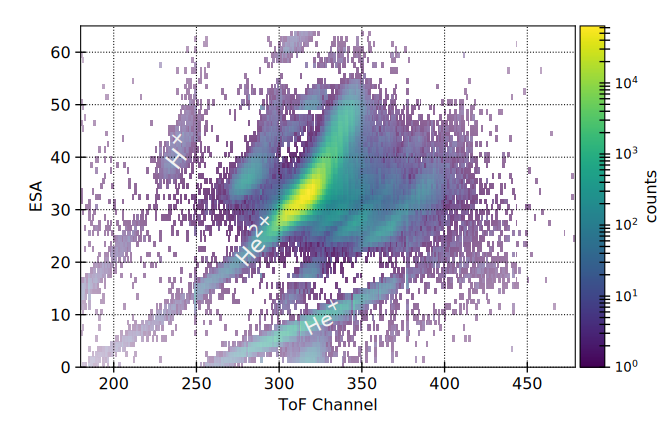
\includegraphics[scale=0.65]{Pics/epq_rng0.pdf}
	\column{3.5cm}
	\vspace{-3.5cm}
	\begin{mdframed}[roundcorner=4pt,userdefinedwidth=3cm,
		align
		=center,
		linecolor
		=black,backgroundcolor=blue!8,
		linewidth
		=1pt]
		$\frac{E}{q} = \frac{1}{2} \, \frac{m}{q} \, v^2$
	\end{mdframed}
	\begin{mdframed}[roundcorner=4pt,userdefinedwidth=3.5cm,
		align
		=center,
		linecolor
		=black,backgroundcolor=blue!8,
		linewidth
		=1pt]
		$\left[\frac{m}{q}\right]_{He^+} = 4 \frac{amu}{C}$
	\end{mdframed}
\end{columns}
\end{frame}



%%%
\begin{frame}{EpQ measurement}
	\vspace{-.25cm}
	\begin{columns}
		\column{4.5cm}
		\only<3>{\vspace{1.5cm}}
		\begin{figure}									
		\only<1,2>{\includegraphics[scale=0.14]{Pics/swics_sensor_flipped_rotated_arrows.pdf}} 
		\only<3>{\includegraphics[scale=0.2]{Pics/sw_pui_gloeckler.png}}
		\caption{\tiny{\begin{center}
					\textit{Gloeckler, Geiss et al., 1992}\end{center}}}	
				
		\end{figure}
		\column{4cm}
		\only<1>{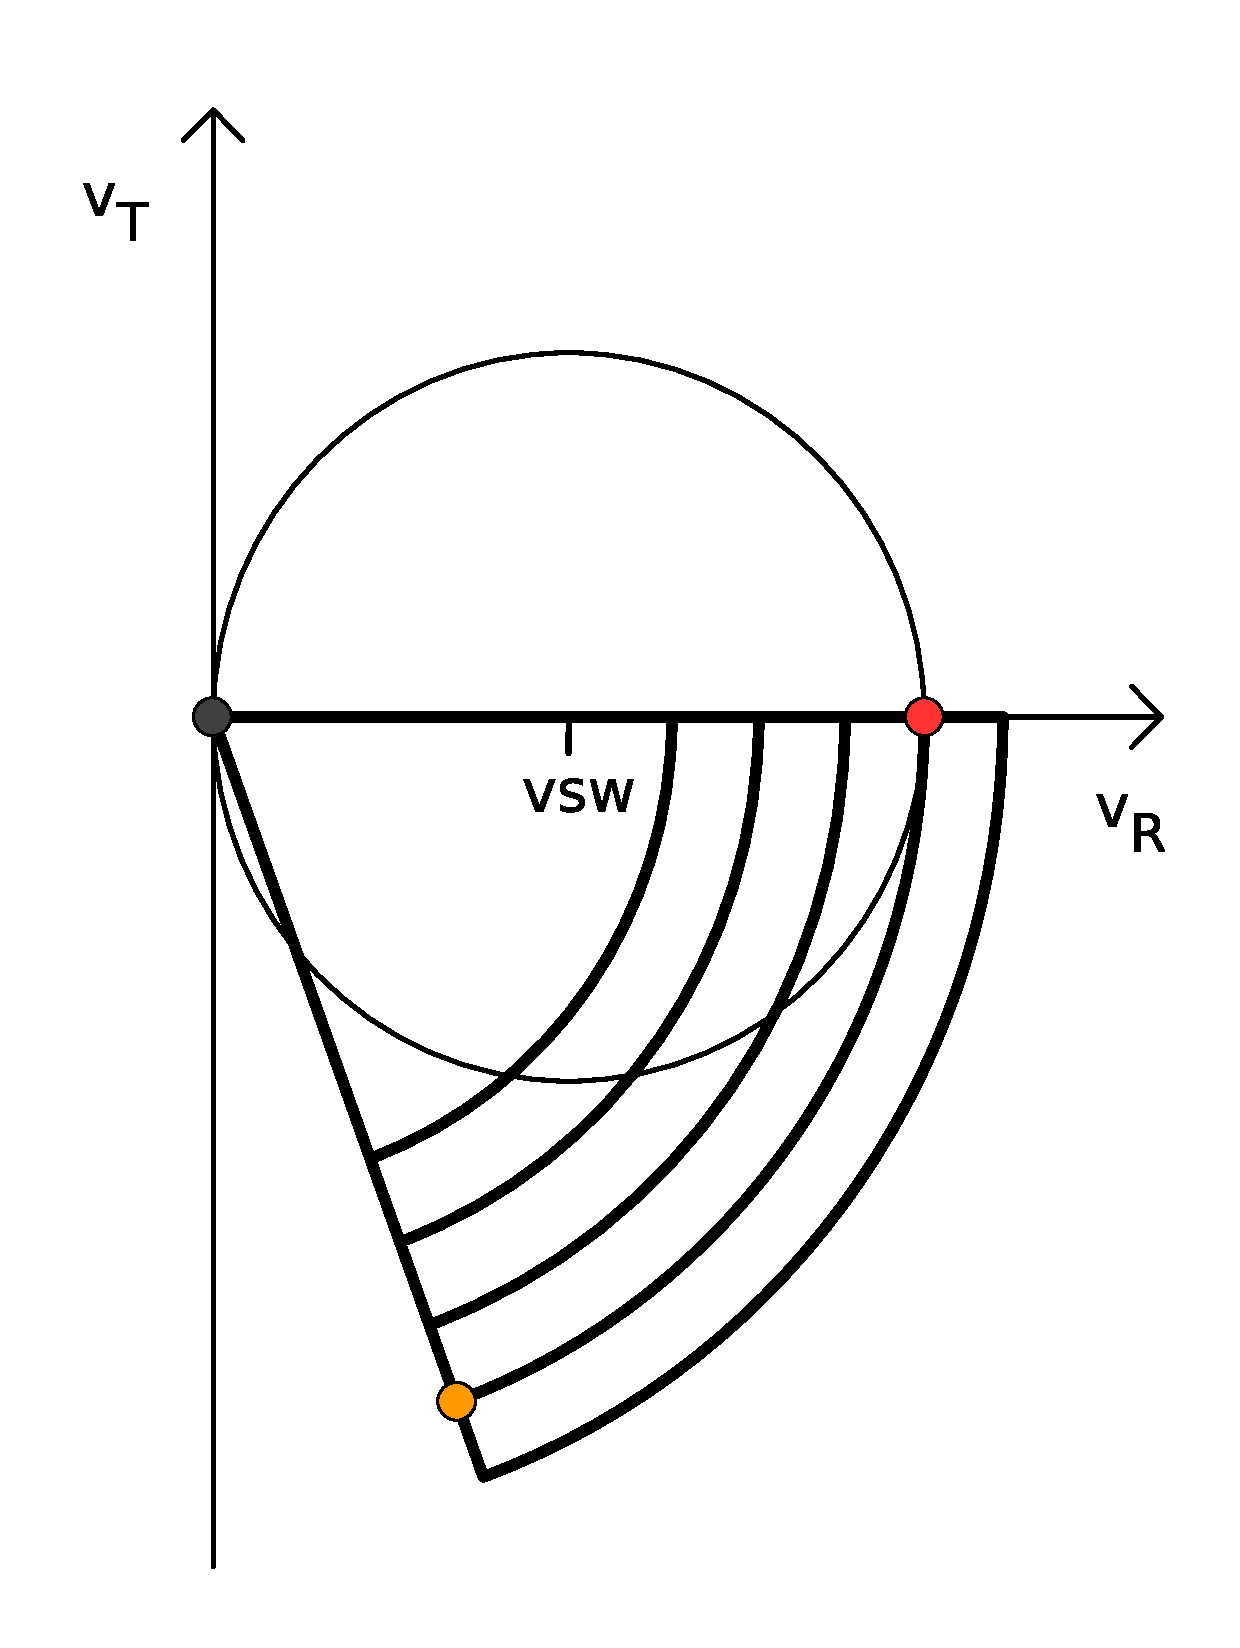
\includegraphics[scale=0.24]{Pics/swics_collimator111.pdf}}
		\only<2,3>{\includegraphics[scale=0.24]{Pics/swics_collimator22.pdf}}
	\end{columns}
	\begin{itemize}
		\item For constant $\frac{m}{q}:$ $\frac{E}{q}$-step $\widehat{=}$ absolute value of velocity
		\only<3>{\item Integration over EpQ shells $\rightarrow$ loss of information!}
	\end{itemize}
\end{frame}
%%%
\begin{frame}{Angular resolution}
	\vspace{-.22cm}
	\begin{columns}
		\column{4.5cm}
		\begin{figure}									
			\includegraphics[scale=0.14]{Pics/swics_sensor_flipped_rotated_ellipse.pdf}
			
		\end{figure}
		\column{4cm}
		%\vspace{1.1cm}
		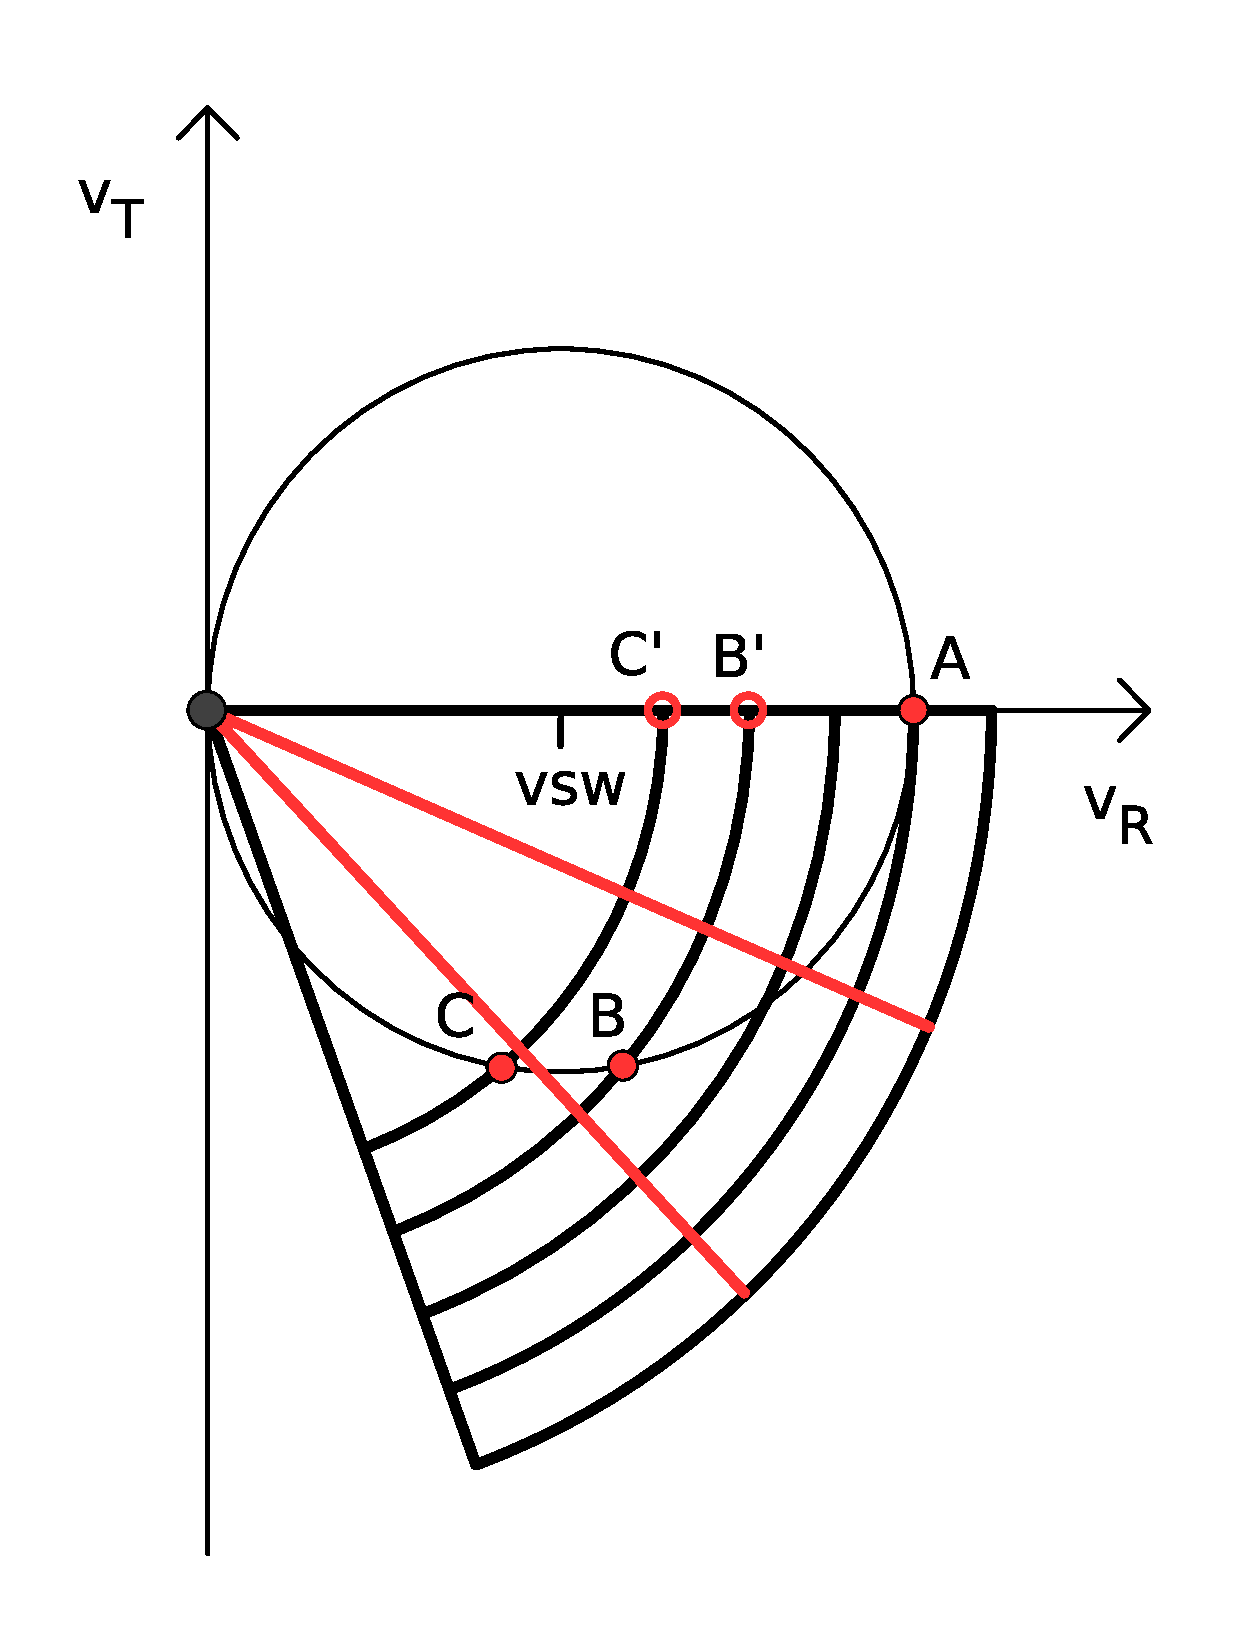
\includegraphics[scale=0.24]{Pics/swics_collimator33.pdf}
	\end{columns}
	\begin{itemize}
	\item SWICS: \textbf{3 detectors} \\ \small{Rough distinction between angles of incidence}
	\item \normalsize{3rd dimension: spin of the SC} \\ \small{Divided into \textbf{8 sectors}}
\end{itemize}
\end{frame}

%%%
\begin{frame}{Virtual Collimator}
	\begin{columns}
		\column[]{7cm}

		\includegraphics[scale=0.35]{Pics/coll_1sec.pdf}
		\column[]{7cm}
		\includegraphics[scale=0.35]{Pics/coll_allsec.pdf}
	\end{columns}
	
\end{frame}
%%%

%%%


\begin{frame}{}
\includegraphics[scale=0.35]{Pics/coll_3shells.pdf}
\end{frame}

%%%


\begin{frame}{}
\begin{figure}
	\includegraphics[scale=0.3]{Pics/RTN_AA.pdf}
\end{figure}
\end{frame}

%%%

\begin{frame}{}
\begin{figure}
	\includegraphics[scale=0.3]{Pics/aa_new.pdf}
\end{figure}
\end{frame}

%%%

\begin{frame}{}
\begin{columns}
	\column[]{6.cm}
		\begin{figure}
			\includegraphics[scale=0.4]{Pics/coll_aa.pdf}
		\end{figure}
	\column[]{7.5cm}
		\begin{figure}
			\includegraphics[scale=0.4]{Pics/hist_det_sec_aa_90days2001.pdf}
		\end{figure}
\end{columns}
\end{frame}

%%%

\begin{frame}{Transition}
\begin{columns}
\column[]{5cm}
\vspace{-1cm}
	\begin{figure}
		\includegraphics[scale=2.0]{Pics/vspace_sc_trans.pdf}
	\end{figure}
	\vspace{-1cm}
	\begin{figure}
	\includegraphics[scale=2]{Pics/vspace_sw_trans.pdf}
\end{figure}


\column[]{6.2cm}
	\vspace{3.5cm}
	\begin{figure}
		\includegraphics[scale=2]{Pics/wspace_sw_trans.pdf}
	\end{figure}
\end{columns}
\end{frame}

%%%

%%%

\begin{frame}{Slice Counts}

\end{frame}

%%%


%%%

\begin{frame}{Einschub: Counts zu PSD}
	\begin{figure}
	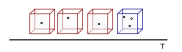
\includegraphics[scale=.6]{Pics/norm_time.pdf}
\end{figure}
\end{frame}

%%%

\begin{frame}{Slice PSD}

\end{frame}


%%%

\begin{frame}{Skymap}

\end{frame}



%%%

\begin{frame}{1D}

\end{frame}






\section{Outlook \& Conclusion}
%%%

\begin{frame}[plain]{Conclusion}

\end{frame}

%
%
%
\section{Motivation}
\section{kurze Wdh PUIs}
\section{SWICS}

\section{Outlook}
\section{Summary}
%
%
%
\end{document}